\documentclass{article}
\usepackage{graphicx} % Required for inserting images
\usepackage[natbibapa]{apacite}
\usepackage[colorlinks=true,linkcolor=black,citecolor=black,urlcolor=black]{hyperref}


\title{\vspace{-2cm}Assignment 1\\
    The Scientific Discourse}

\author{Tymur Mykhalievskyi\\ 7031100}
\date{\today}


\begin{document}

\maketitle

\section{General Overview}


\section{MIC}
In this section we will share my thoughts on MIC. The overall idea seems promising on the first glance. MIC is supposed to be the one metric that is general and equitable (according to the definition by \cite{reshef2011}). Firstly reading the work by \cite{reshef2011}, prima facie, MIC completely satisfies these properties. In particular, MIC does not make any assumptions about the underlying funciton which is supposed to make it generalize very well. However, after reading the concerns presented by \cite{simon2014} and \cite{kinney2014}, a more thorough analysis of MIC had to be conducted.

\subsection{Limitations of MIC}

\subsubsection{Grid Resolution}

\subsubsection{Geometrical Interpretation of MIC}
The underlying implementation of MIC is based on the idea of partitioning the scatter plot of two variables into a grid. At this point we can see an important limitation of MIC which also does not align with the equitability of the metric. Due to the fact that the grid is made of rectangles, the relationship some relationships between two variables could work particularly well. For example, if the underlying function is a step function, the grid would capture the relationship very well. However, if we exchange the underlying function to a modular function, the grid would not be able to capture the realtionship as well. This is because the step function would be able to fit into the grid cells very well, while the modular function being not parallel to any of the axis would not be able to fit into the grid cells. This parituclar case is visualized in \autoref{fig:step_mod}

\begin{figure}
    
    \centering
    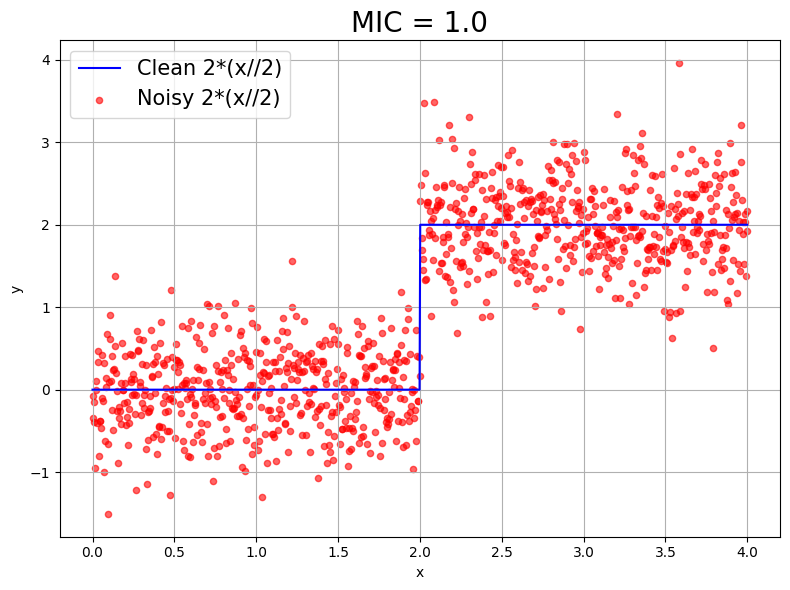
\includegraphics[width=0.47\textwidth]{images/step1.png}
    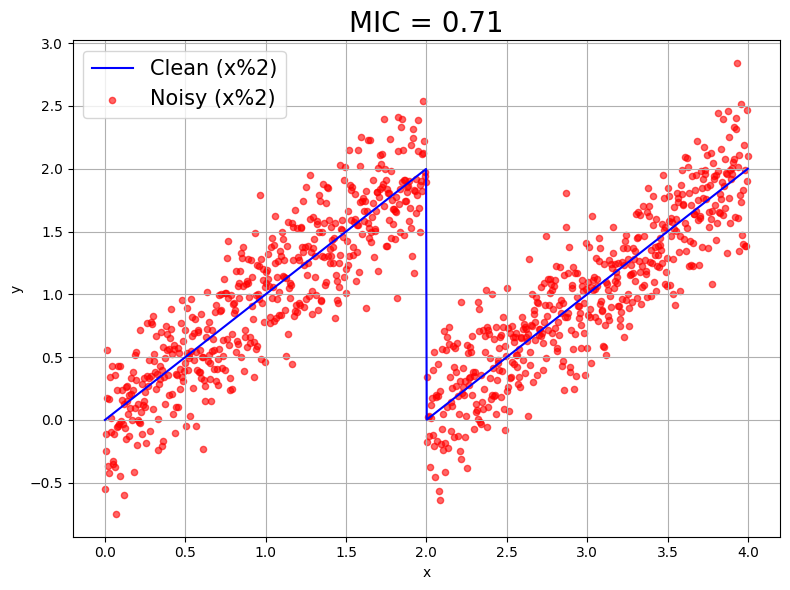
\includegraphics[width=0.47\textwidth]{images/mod1.png}
    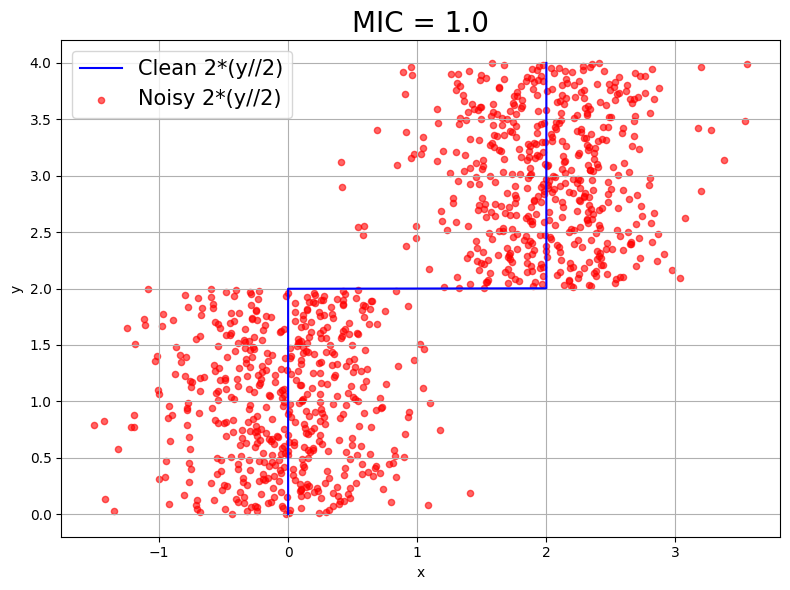
\includegraphics[width=0.47\textwidth]{images/step2.png}
    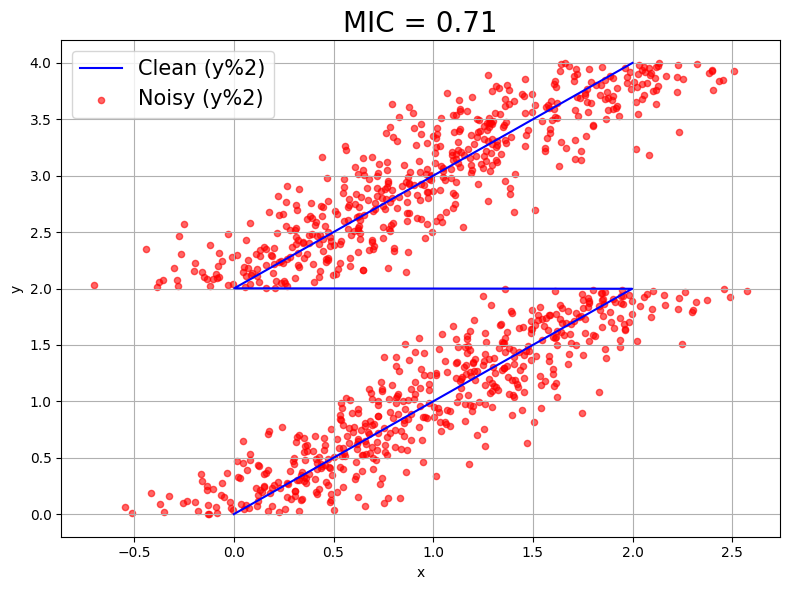
\includegraphics[width=0.47\textwidth]{images/mod2.png}
    \caption{Comparison of the step function and modular function. The left plot shows the step function with its inverse variant on the bottom. While the right plot shows the modular function with its inverse variant. Both plots were generated using the exact same parameters: $n = 1000, 1-R^2=0.2, x\in [0, 4)$. The source code can be accessed via GitHub \citep{src}}
    \label{fig:step_mod}
\end{figure}

\subsection{Why MIC will not be the best}

\section{Equitability}



\bibliographystyle{apacite}	
\bibliography{references}


\end{document}


